\documentclass[english,a4paper,oneside,12pt]{article}

\usepackage[utf8]{inputenc}
\usepackage{supertabular}
\usepackage{fancyhdr}
\usepackage{amsmath}
\usepackage{babel}
\usepackage{hyperref}
%\usepackage{amssymb}
%\usepackage{theorem}
\usepackage{float}
\usepackage{longtable}
\usepackage{color,colortbl}
%\usepackage{verbatim}
\usepackage{babelbib}
\usepackage{pst-all}
\usepackage{graphicx}
\usepackage{geometry}
\usepackage{pdfpages}
\usepackage{framed}
\usepackage{caption}
\usepackage{subcaption}
\usepackage{wrapfig}
\usepackage{pbox}
%\usepackage[onehalfspacing]{setspace}

\definecolor{tcA}{rgb}{0.627451,0.627451,0.643137}
\renewcommand{\familydefault}{\sfdefault}
\renewcommand{\arraystretch}{1.2}
\newcommand{\settocdepth}[1]{\addtocontents{toc}{\protect\setcounter{tocdepth}{#1}}}

% -------------------- Seitengroessen ----------------------

%\addtolength{\topmargin}{2cm}
\geometry{a4paper,top=35mm,left=25mm,right=25mm,bottom=25mm,headsep=10mm,footskip=12mm}
\setlength{\parskip}{1ex plus 0.5ex minus 0.2ex}


% -------------------- Kapitelangabe oben ----------------------

\pagestyle{fancy} % Dieser Befehl muss nach (!) \textwidth stehen!
\cfoot{}
%\renewcommand{\sectionmark}[1]{\markboth{#1\ }{}}

\fancyhf{} %alle Kopf- und Fußzeilenfelder bereinigen
\fancyhead[OL]{\leftmark} %Kopfzeile links
\fancyhead[OC]{} %zentrierte Kopfzeile
\fancyhead[OR]{\thepage} %Kopfzeile rechts
\fancyhead[EL]{\thepage} %Kopfzeile links
\fancyhead[EC]{} %zentrierte Kopfzeile
\fancyhead[ER]{\leftmark} %Kopfzeile rechts


\begin{document}
\pagenumbering{roman}

%--------------- Vorspann ----------------------------------

\thispagestyle{empty}
\newcommand{\mc}[3]{\multicolumn{#1}{#2}{#3}}
\newcolumntype{R}[1]{>{\raggedleft\arraybackslash}p{#1}}

\begin{center}
%\begin{tabular}{lr}\hline
%     \begin{minipage}{7cm}
%        \begin{center}
%           \vspace*{3ex}
%           Softwarepraktikum
%           \vspace*{3ex}
%           VIS Institut Universität Stuttgart
%           \vspace*{3ex}
%        \end{center}
%     \end{minipage}
%   & \mc{1}{l|}{
%   \begin{minipage}{7cm}
%      \begin{center}
%         \vspace*{3ex}
%         Rechtsobentext
%         \vspace*{3ex}
%         Stuttgart
%         \vspace*{3ex}
%      \end{center}
%   \end{minipage}
%   }\\\hline
%\end{tabular}
%\begin{tabular}[t]{p{0.3\textwidth}|r}
%\begin{tabular}{|p{.5\linewidth-2\tabcolsep}|r{.5\linewidth-2\tabcolsep}|}
%   \hline
%   Softwarepraktikum \newline Institut für Visualisierung \newline Universität Stuttgart & 
%   
\includegraphics[width=3cm]{images/vislogo}
%   \\ \hline
%\end{tabular}
\begin{figure}[t]
\vspace*{-1.4cm}

   \begin{minipage}[t]{6cm}
    \vspace{5pt}
      Softwarepraktikum at\newline Visualization Research Center \newline University of Stuttgart

   \end{minipage}
   \hfill
   \begin{minipage}[t]{6cm}
      \vspace{0pt}
      \includegraphics[width=5.5cm]{images/visuslogo}

    \end{minipage}
\end{figure}
%   
\includegraphics[width=3cm]{images/vislogo}
\begin{minipage}{13cm}
\begin{center}
\vspace*{8ex}
\large
Softwarepraktikum\\
\vspace*{1cm}
\Huge
\textbf{TrackIt\\ \vspace*{-1mm} - \\ \vspace*{-1mm} \large Video Ground Truth Editor}\\
\vspace*{1cm}
\normalsize
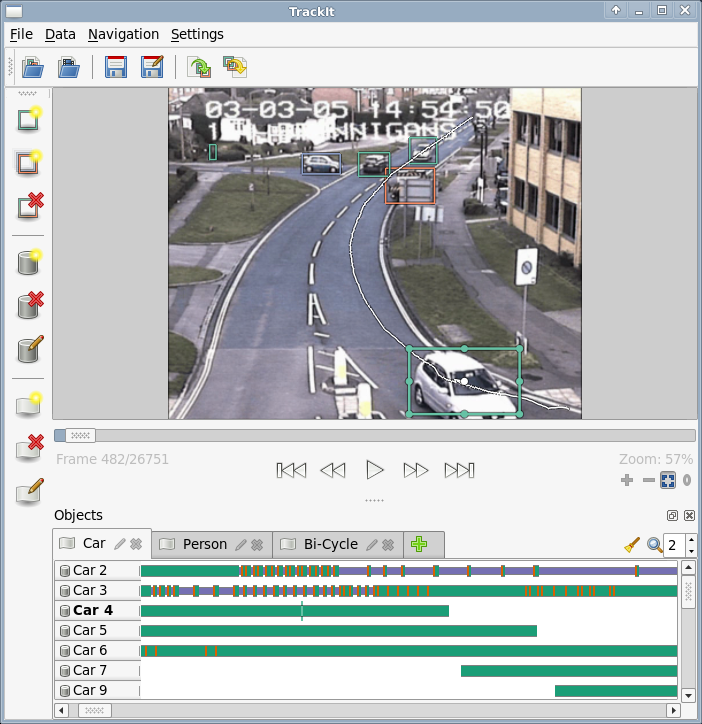
\includegraphics[height=8cm]{images/Titelbild}
\end{center}
\vspace{1cm}
\renewcommand{\arraystretch}{1.6}
\enlargethispage{1.5cm}
\begin{tabular}{ll}
Programming and Documentation: &Sven Klingel\\ & (\href{mailto:klingesn@studi.informatik.uni-stuttgart.de}{klingesn@studi.informatik.uni-stuttgart.de})\\
Programming and Documentation: &Hanspeter Haegele\\& (\href{mailto:haegelhr@studi.informatik.uni-stuttgart.de}{haegelhr@studi.informatik.uni-stuttgart.de})\\
Supervision:                     &Kuno Kurzhals:\\& (\href{mailto:kuno.kurzhals@vis.uni-stuttgart.de}{kuno.kurzhals@vis.uni-stuttgart.de})

\end{tabular}
\vspace{1ex}
\end{minipage}
\end{center}

      % Titelseite
\clearpage

\tableofcontents 
\newpage

%\fancyhead[OL]{VORWORT}
%\include{Vorwort}
%\clearpage

%--------------- Hauptteil  (max. 30 Seiten) --------------

\pagenumbering{arabic}

\fancyhead[OL]{\leftmark}
\section{The Program}
   \subsection{Introduction}
   TrackIt is a program to enable users to easily apply bounding boxes (henceforth abbreviated with \emph{bboxes}) on video files to create ground truth data for those files. Videos are opened with the use of the OpenCV framework, painting Bboxes is done via the QT Framework and OpenGL. Keyboard shortcuts assist in efficient working and data manipulation. All used file-formats are well-documented. We hope we created an easy-to-use, reliable and robust program.

\section{Using TrackIt}
%%%%%%%%%%%%%%%%%%%%%%%%%%%%%%%%%%%%%%%%%%%%%%%%%%%%%%%%%%%%%%%%%%%%%%%%%%%%%%%%%%
The main purpose of TrackIt is to assist the user in manually generating bounding box data for videos to supply tracking information for other programs, create ground truth for visual studies or similar purposes. Here comes a step-by-step introduction and overview, showing all steps necessary to create tracking data by hand. You can move and rearrange all widgets freely, not limited to inside the main windows, which is especially useful in dual-screen setups.

\subsection{Starting TrackIt}
Under Linux we recommend starting TrackIt from a terminal, as the underlying OpenCV framework and video codecs might dump useful information to standard output.\\
Under Windows, just doubleclick the executable TrackIt.exe.

   
\subsection{Opening Video Files}
%todo 
      Most likely you'll start with a video file containing some features you want to track manually: Press „File $\rightarrow$ Open Video“ and a file dialog window will appear. Navigate to your video file and press open. You will be provided with a standard category and object, so you can just start creating Bboxes.\\
\\
   \begin{tabular}[H]{|p{0.95\textwidth}|}
   \hline
Tip (Linux): FFMpeg, the underlyling video decoder used by TrackIt might in some cases dump information about wrongly encoded video files to console. Some of them may result in your tracking results to be not in sync  with the actual video data. Hence we recommend starting TrackIt in a terminal.\\
   \hline
   \end{tabular}


\subsection{Navigating in Video Files in the Video Window}
\begin{figure}[t]
\centering
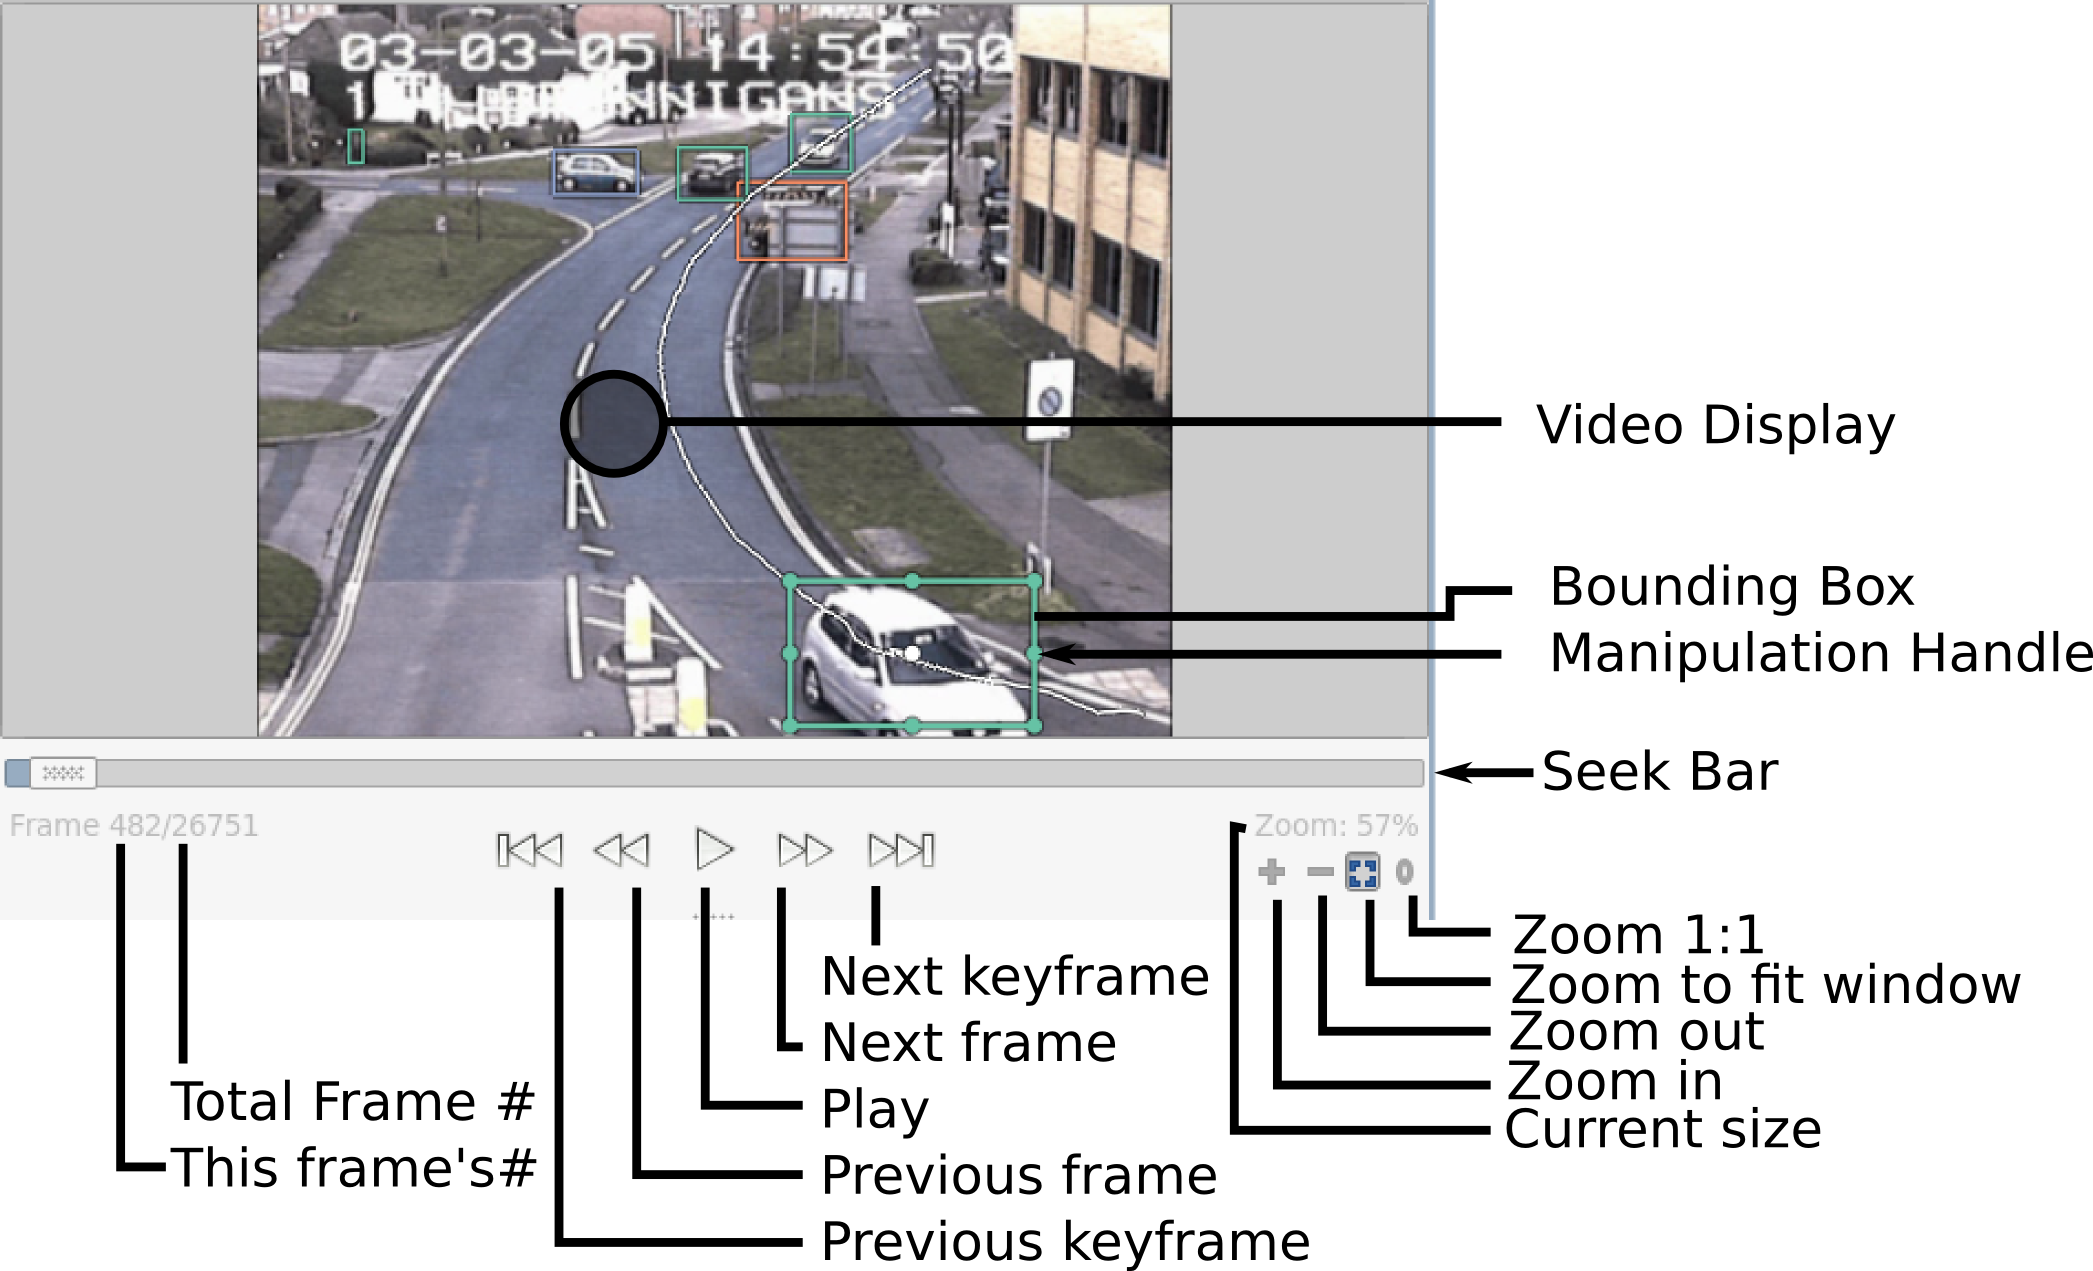
\includegraphics[angle=0,width=0.95\textwidth]{images/videowindow_final}
\caption{Video window}
\label{fig:videowindow}
\end{figure}
The controls in the lower middle are for navigating. 
Pressing the \emph{Play/Pause}-button will make the program play continuously at the framerate of the video, the "\emph{previous frame}" and "\emph{next frame}" buttons will always just play one frame forwards or backwards. Contrary to this, the "\emph{Next Keyframe}"-button will jump to the next keyframe of the currently selected object (yet only if there are actually keyframes before or after).\\
You can directly jump to any part of the video via clicking on any point of the \emph{seek bar}, or grabbing the slider and dragging it to the desired position. The Framecount on the lower left meanwhile indicates the framenumber and the total number of frames.\\
The lower right section of the Video window contains the zoom buttons to control the video's size. Enlarge the video size with the "\emph{+}" button, shrink it with the \emph{-} button. The other two buttons control fitting to window dimension size and 1:1, meaning that one pixel in the video is one pixel on the screen.

\subsection{Opening \& importing Tracking Data Files}
TrackIt supports various types of Tracking data, ViPER being one of the most commonly used ones. To open a Data file, click on "File $\rightarrow$ Open" and choose your .btd file.\\
If you want to open files of other file types, such as \emph{.bb} or a \emph{ViPER .xml} file, you must use "File $\rightarrow$ Import". After opening a data file, TrackIt will automatically look for a video file with the same file name or a video file name specified in the meta data of a ViPER file and try to open it. 


\subsection{Data window}
\begin{figure}[t]
\centering
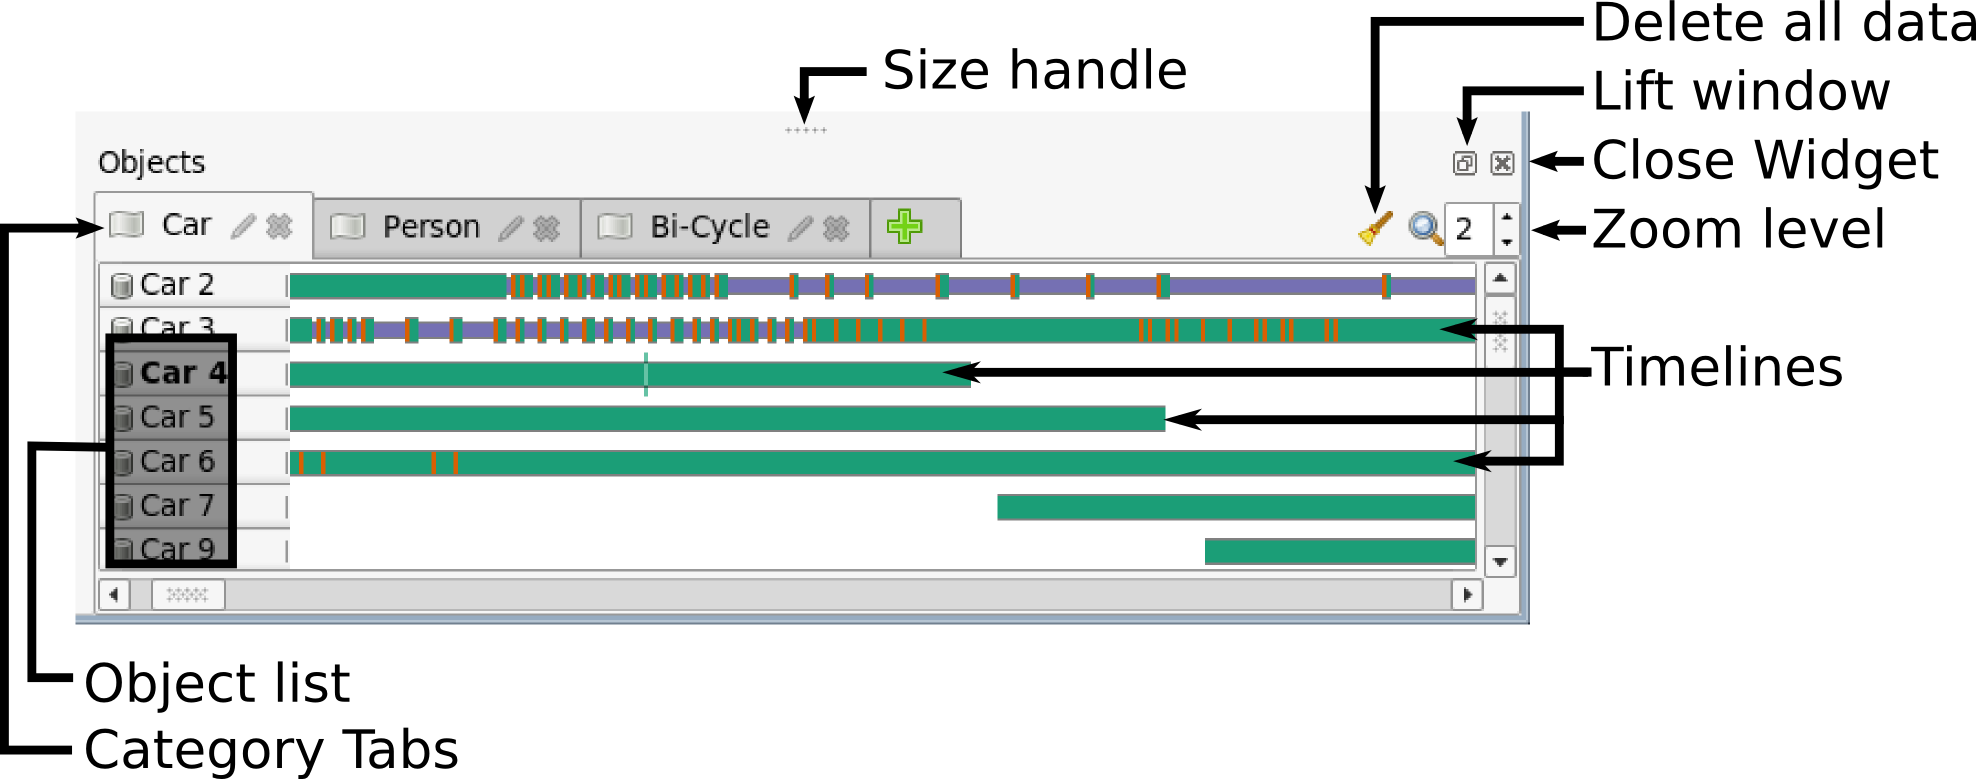
\includegraphics[angle=0,width=0.95\textwidth]{images/datawindow_final}
\caption{Data window}
\label{fig:datawindow}
\end{figure}

The \emph{data window} contains a view of all the data that has already been created or loaded.
At first, let's focus on the general handling of this window. As shown in figure \ref{fig:datawindow}, you can enlarge and shrink the the window by dragging the \emph{size handle} on the very top center. The upper right corner holds the controls to close or to detach the window from the main window. This makes it easy to use our program in dual-monitor setups and the like.\\

On the top there are the \emph{Category Tabs}, which allows you to organize your objects. Each tab contains (from left to right):
\begin{description}
   \item[Flag-symbol] Indicates it's a group.
   \item[Category name] All objects in this Category will carry this Name, along with a number.
   \item[Pen] Edit the Name of the category.
   \item[X] Delete Category and all it's content (You will be asked to confirm this step).
\end{description}

Left hand side there are the labels of objects. Directly right of each label there's the timeline.  To transfer an object to another category, right-click the object's label or timeline, select "Object.. $\rightarrow$ Move object" and select the category.\\
A timeline shows the bboxes of each object, sorted by frame number. Figure \ref{fig:timeline} shows several different objects and box types. Here you can mark and delete several bounding boxes at the same time. While hovering your cursor over any place, the frame number is displayed near the cursor as shown in fig. \ref{fig:timeline_zoomed}, and clicking will jump the video display to the selected frame. Change the timeline scale by using the \emph{zoom level} button on the upper right of the datawidget.
   \begin{figure}[h]
      \centering
      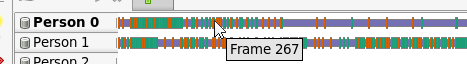
\includegraphics[angle=0,width=0.6\textwidth]{images/timeline}
      \caption{Datawidget's timelines in close up}
      \label{fig:timeline}
   \end{figure}
\enlargethispage{1cm}
   \begin{figure}[h]
      \centering
      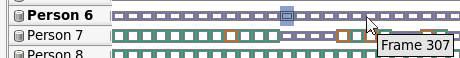
\includegraphics[angle=0,width=0.6\textwidth]{images/timeline_zoomed}
      \caption{Data window's timelines after using the zoom button}
      \label{fig:timeline_zoomed}
   \end{figure}
\newpage
\subsection{The action bar}
   \begin{wrapfigure}{l}{4.5cm}
         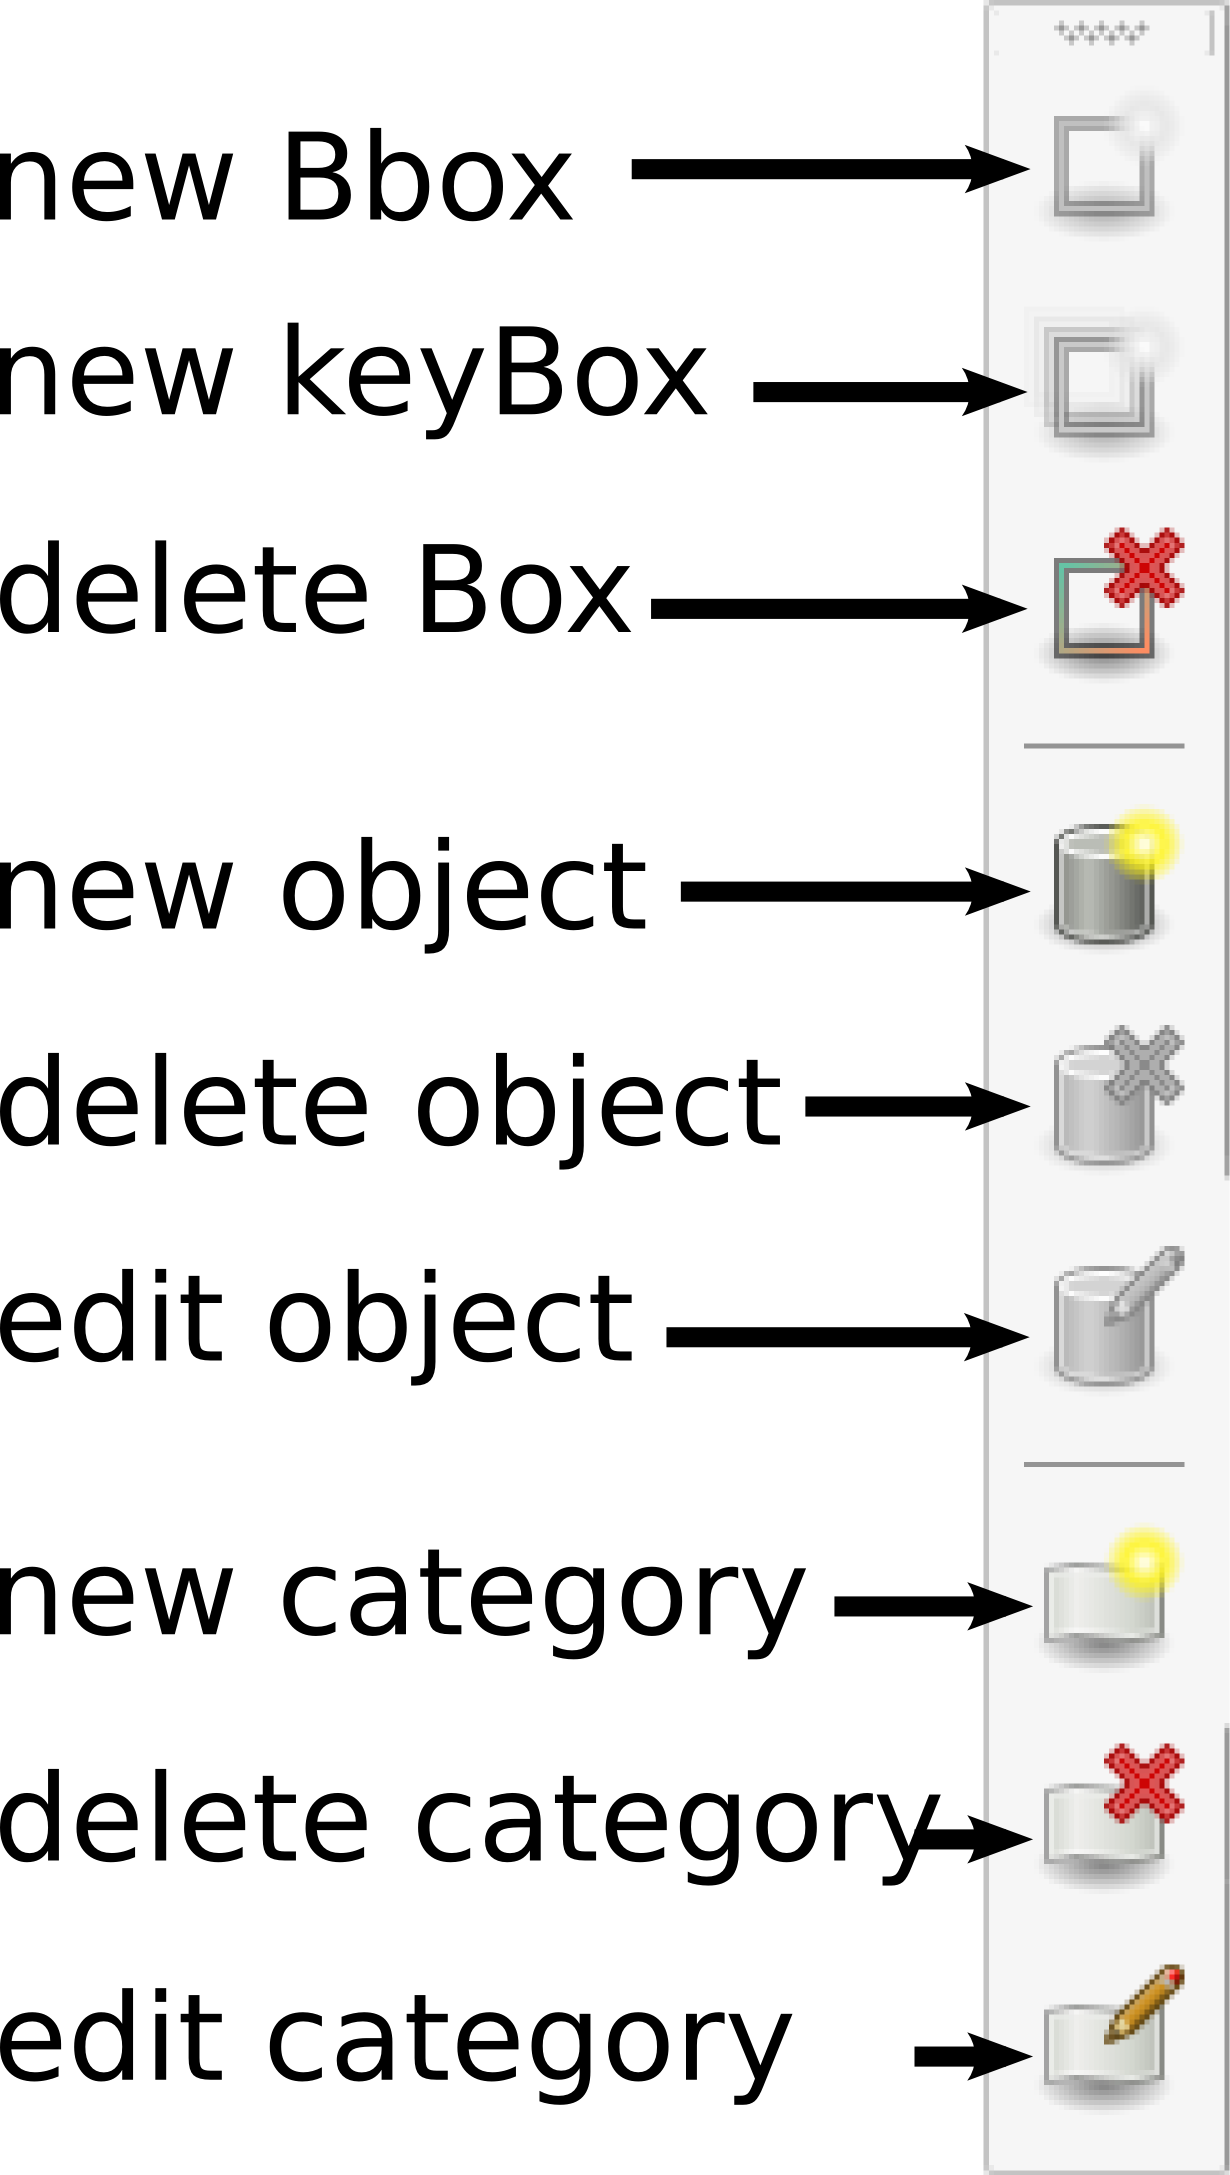
\includegraphics[width=4cm]{images/actionbar_final}
      \caption{Action Bar}
      \label{img:actionbar}
      \vspace{-1cm}
   \end{wrapfigure}
 The \emph{action bar} is located at the left edge and contains the controls (buttons) to create, delete or modify bboxes (first group of icons from top), objects (second group from top, and groups (bottom), as explained in figure \ref{img:actionbar}. The use of these buttons/functions is thoroughly explained in sections \ref{sec:bboxes} and \ref{sec:groupsandobjects}. The most commonly used actions such as \emph{bbox} creation ("R" key), \emph{keybox} creation ("F" key) and Object creation (Ctrl+R) are also available as keyboard shortcuts, see Appendix B table \ref{movieactions}.
%todo hier bild
\subsection{Creating a Bbox}
\label{sec:bboxes}
Suppose we have an object we want to track and we see it displayed in the video window in the actual frame. To create a Bbox, simply click the green Bbox-button in the left menu and your cursor will turn to a crosshair when it's in the video window. Now simply left-click and while holding the mouse button down, drag a bounding box around your desired object. \\
Does not look exactly as you wanted? On the edges and corner of the activated bounding box are enlarged blobs, called „handles“. With those handles you can adjust the size of the keybox. By clicking inside the box and holding your mouse button down, you can also change its position. Finally you can advance one frame further, and track your object the same way in the this frame.\\
By clicking at any Bbox in the window it will be marked as activated (its frame will become thicker) and you will be able to manipulate it. Also you will see that the mark in the data window jump to the right category and object, showing to which object the bounding Box belongs to.

   \subsubsection{Types of BBoxes}
      There is not only one kind of bounding Boxes, but several which serve different purposes.
      \begin{description}
         \item[Single BBox]The most usual bboxes are „single-frame“ bboxes, valid for one frame, like the one you encountered in the example above, they are usually depicted in green.
         \item[Key BBox]Key Bboxes are a concept to make it easier tracking an object's linear movement. It will be explained thoroughly in section \ref{interpolation} 
         \item[Virtual Keyboxes]Virtual Bboxes are bounding boxes, that are linearly interpolated. Their position and size depends only on a normal Bbox (or keybox) before and the keybox after them. You can not directly manipulate a virtual keybox, but you can convert it to a Key- and SINGLE Bboxes, also explained in \ref{interpolation}. 
      \end{description}


\subsection{Creating a Key Bbox and interpolated „virtual“ frames}\label{interpolation}
If an object moves with a constant direction and speed over several frames, you can save time by using linear interpolation between bounding boxes of the same object. So let's assume you have an object like a car passing through your video from left to right at a constant speed. Instead of generating a \emph{bbox} for each frame you scroll to the end of the constant motion of this object. By clicking the orange rectangle in the \emph{action bar}, a bounding box appears at the original place, and you can fit it to the position (and size) of the moving object. In the datawindow, you can then see the (now selected) orange \emph{keybox}, and left of it, the violet "\emph{virtual bboxes}".
\\
Play the scene again, and you will see that the last box will transform in position and size along a path from the last created \emph{bbox} towards the created \emph{keybbox}.
You can not directly edit a virtual keybox, but by selecting it in the data (or, of course, video) window, and pressing the "\emph{convert keybox}" (former \emph{create keybox}) button, you can convert it to an editable type of bounding box while preserving linear interpolation before and after.
%\vspace*{-0.3cm}
\begin{figure}[H]
   \begin{tabular}{|p{0.95\textwidth}|}
   \hline
   Tip: Object is not transforming and not moving, but still there? "Not moving" is a constant movement at zero speed, so you can just create a Key-BBox.\\
   \hline
   \end{tabular}
\end{figure}

\subsection{Objects and groups}
\label{sec:groupsandobjects}
  Each object has exactly one \emph{bbox} per frame. To track more than one video object in one frame you have to create a new data object by clicking on the "create object" button in the action bar, or by using the keyboard shortcut "Ctrl+F".\\
However, with many objects the overview might get cluttered, so grouping of similar objects is recommended, also group membership leads to more semantic information for other programs:
For example, in a ball game, putting all players of team "blue" in ne ogroup and all "red" players in another. \\ To move an object into another group, right-click on the object, select "Object... $\rightarrow$ Move object". To switch categories use the "Q" and "E" keys.

\subsection{Opening/Saving and importing/exporting data files}
To save a file, press "File $\rightarrow$ Save data" or "File $\rightarrow$ Save data as...". Give a filename, and chose your data format from the selector and click okay.
Now let's explain the very important distinction between opening/saving and importing/exporting: Opening and saving will always preserve all features TrackIt has. However, importing and exporting wil always come along with a loss of meta-information, such as group membership or group name, yet no bounding box data will be lost. For more information see \ref{fileformats} in Appendix A.

\subsection{Keyboard controls for efficiency}
Using Keyboard controls can greatly improve your working efficiency.  We'll just show some basic usage, a table with all available keys and secondary keyboard layouts can be found in tables of \ref{fileactions} in Appendix B .\\
Use "D" and "A" key to jump one frame forward or respectively backward, and the "W" and "S" key to select the next / previous object. In the data window, this corresponds to left-right/up-down movement of the selection. "Q" and "E" will allow you to easily switch categories, while "R" and "F" create new bboxes, respectively key boxes, so your mouse pointer can rest over the objects and do the manipulation, while the hand resting on your keyboard selects the action type.
Zooming in the Video is avaiblable by holding down the Ctrl key and either pressing the "+" or "-" keys, or easier by holding down the Ctrl key and scrolling your mousewheel up or down.



 
\clearpage

\appendix
\fancyhead[OL]{APPENDIX}
\addcontentsline{toc}{section}{Appendix}
\section{Appendix A}
   \subsection{File Formats}
      \label{fileformats}
      TrackIt supports a the following file formats currently supported file Formats include:\\
      .bb, .btd, ViPER .xml  
      However, not all file formats support all features of the other file formats or our program, loss of grouping and naming information may occur. however, there is never any loss of Bbox information.
      This table shows which file formats support which features, the features being listed as:
      \begin{description}
         \item[Categories]One or more objects may be put together in a category tab, to simplyfy grouping objects.
         \item[Holes] Allows objects to have frames with no bounding boxes between two frames with bounding boxes. If holes are not supported, objects will be split.
         \item[Named Categories]Not only grouping information is saved, but also a label to each group, like „car“ and „persons“, or „animals“. If this is not possible, groups will be saved without a group name.
         \item[Object names] Give Objects name instead of just a random number within their group.
         \item[Keyframes] Supports saving of keybboxes and linearly interpolating in between them. If not possible to save keybboxes, these and their associated virtual Bboxes will be converted to single Bboxes.
         \item[Run-length-encoding] Run-length-encoding saves space by saving the bbox position,first appearance and the duration of its presence there. If RLE is not possible, BBoxes will be converted to single keyboxes.
      \end{description} 

   \begin{table}[H]
    %todo: sowohl überschrift als auch table linksbündig?
     \centering
     \label{features} 
     \caption{supported features by File format}
      \begin{tabular}[]{|l|c|c|c|c|c|c|}
         \hline
%                 &           &            &            &            \\  
                 & Categories&  Holes     & Named Cat. & Obj. Names & Keyframes  & RLE\\\hline
         .btd    &    X      &   X        &     X      &            &     X      & \\\hline
        ViPer XML&    X      &   X        &     X      &          &              &  X \\\hline
        .bb      &           &            &            &            &           &  \\\hline
         \hline
      \end{tabular}
   \end{table}
  
   \subsubsection{.btd}
      BTD (binary tracking data) is our own data format and therefore capable of saving all TrackIt data without any loss. The Data is saved in binary mode using QDataStream's serialization mechanisms in version 12 so it can be written and read on any platform where Qt is available. \\
      The actual serialization of our internal data structure is specified in table \ref{tab:btdformat}.  For details on the serialization of Qt's own types like QString or QList see \href{http://qt-project.org/doc/qt-4.8/datastreamformat.html}{http://qt-project.org/doc/qt-4.8/datastreamformat.html}.


      \begin{table}[h]
         \centering
         \caption{BTD file format}
         \begin{tabular}{|l|l|}
            \hline
            \textbf{Type} & \textbf{Description} \\
            \hline\hline
            quint8 & Part of magic number, must be 0x42 ('B') \\
            \hline
            quint8 & Part of magic number, must be 0x54 ('T') \\
            \hline
            quint8 & Part of magic number, must be 0x44 ('D') \\
            \hline
            quint8 & BTD version (currently 1) \\
            \hline
            QString & Filename of the associated video file \\
                    & (can also contain a relative or absolute path) \\
            \hline
            quint32 & Current ID of the ID counter \\
                    & (Last assigned ID + 1) \\
            \hline
            QList<Category> & Categories \\
            \hline \hline
            \multicolumn{2}{|c|}{\textit{Category}} \\
            \hline
            QString & Name of the category \\
            \hline
            QList<Object> & Objects \\
            \hline \hline
            \multicolumn{2}{|c|}{\textit{Object}} \\
            \hline
            quint32 & ID of the object \\
            \hline
            QList<BBox> & Bounding Boxes \\
            \hline \hline
            \multicolumn{2}{|c|}{\textit{BBox}} \\
            \hline
            quint8 & Type (1=single, 2=key) \\
            \hline
            quint32 & Framenumber \\
            \hline
            QRect & Position and size \\
            \hline
         \end{tabular}
         \label{tab:btdformat}
      \end{table}
  \subsubsection{ViPER xml File} 
Open-standard xml document format introduced by the ViPER-toolkit.\\
(see \href{http://viper-toolkit.sourceforge.net/}{http://viper-toolkit.sourceforge.net/}) This file format is more thoroughly described in\\
 \href{http://viper-toolkit.sourceforge.net/docs/file/}{http://viper-toolkit.sourceforge.net/docs/file/}.
.

   \subsubsection{BB Files}
   BB Files have a simple parsable file format. The first line containes the number of frames, followed by a list of all frames. Each of these frames consists of the numbers of objects that appear in this frame, followed by an object definition, or nothing in case the number of objects is "0". Each object definition contains its lifetime in frames (its first appearance is determined by the framenumber that holds its data), followed by a (possibly empty TODO: Möglich? ) list of bounding boxes. Each bounding Box consists of four integers: distance to top border of video, then distance to left border of video, width and height of video. The EBNF definition puts bb files in a more formal format: 
Unfortunately, BB Files allows only saving of bboxes for consecutive frames for an object, so if there are "holes" without a bbox in between, this object will be split into as many new objects. as it takes to create only objects with consecutive frames.
\begin{table}
  \centering
  \label{bbfiledef} 
  \caption{BB File definition}
   \begin{tabular}[h]{l@{}cl}
      BBFILE   & ::=  & NUMBER\_OF\_FRAMES „$\backslash$n“          \\
               &      & LIST\_OF\_ALL\_FRAMES            \\
      LIST\_OF\_ALL\_FRAMES   & ::= &  NUMBER\_OF\_OBJECTS „$\backslash$n“\\
               &      &       (OBJECT\_DEFINITION $|$ $\varepsilon$) \\
      OBJECT\_DEFINITION  & ::=  & LIFETIME\_IN\_FRAMES „$\backslash$n“ \\
               &      & LIST\_OF\_BBOX                   \\
      LIST\_OF\_BBOX & ::=  & BBOX „$\backslash$n“                  \\
               &     &   (LIST\_OF\_BBOX $|$ $\varepsilon$)       \\
      BBOX     & ::= & NUMBER "\textvisiblespace" NUMBER "\textvisiblespace" NUMBER "\textvisiblespace" NUMBER \\
           &   &// first number: Distance in pixels to top border of video  \\
           &   &// second number: Distance in pixels to the left border.  \\
           &   &// third number: Width in pixels.   \\
           &   &// fourth number: Height in Pixels.  \\
      NUMBER\_OF\_FRAMES & ::=  &  NUMBER\\
      NUMBER\_OF\_OBJECTS & ::= & NUMBER \\
      LIFETIME\_IN\_FRAMES & ::= &NUMBER \\
      NUMBER & ::= & \pbox{12cm}{NUMBER NUMBER $|$ „0“ $|$ „1“ $|$ „2“ $|$ „3“ $|$ „4“ \\$|$ „5“ $|$ „6“ $|$ „7“ $|$ „8“ $|$ „9“} \\
   
%%      // note: The size of LIST\_OF\_BBOXES is the number of frames it appears in after the first frame.
 %%     // note: ALL lists must have all objects in ascending order, even if these objects are empty.
   \end{tabular}
 \end{table} 

%   \verb{BBFILE ::=  NUMBER_OF_FRAMES „\n“      
%                     LIST_OF_ALL_FRAMES    
%   LIST_OF_ALL_FRAMES ::=  NUMBER_OF_OBJECTS „\n“
%                           (OBJECT_DEFINITION | \eps) 
%   OBJECT_DEFINITION  ::=  LIFETIME_IN_FRAMES „\n“ 
%                           LIST_OF_BBOX 
%   LIST_OF_BBOX ::=  BBOX „\n“
%                     LIST_OF_BBOX
%                     | \eps
%   BBOX ::=  NUMBER „ „ NUMBER „ „ NUMBER „ „ NUMBER
%             // first number: Distance in pixels to top border of video
%             // second number: Distance in pixels to the left border.
%             // third number: Width in pixels. 
%             // fourth number: Height in Pixels.
%   NUMBER_OF_FRAMES ::=  NUMBER
%   NUMBER_OF_OBJECTS ::= NUMBER
%   LIFETIME_IN_FRAMES ::= NUMBER
%   NUMBER ::= NUMBER NUMBER | „0“ | „1“ | "2" | „8“ | „9“ 
%
%   // note: The size of LIST_OF_BBOXES is the number of frames it appears in after the first frame.
%   // note: ALL lists must have all objects in ascending order, even if these objects are empty.
%   }

      \begin{table}[H]
         \centering
         \caption{BB file format}
         \begin{tabular}{|l|l|}
            \hline
            \textbf{Type} & \textbf{Description} \\
            \hline\hline
            Integer & Number of frames \\
            \hline
            Frame & First frame \\
            Frame & Second frame \\
            ... & ... \\
            \hline \hline
            \multicolumn{2}{|c|}{\textit{Frame}} \\
            \hline
            Integer & Framenumber \\
            \hline
            Integer & Number of objects starting in this frame \\
            \hline
            Object & First object \\
            Object & Second object \\
            ... & ... \\
            \hline \hline
            \multicolumn{2}{|c|}{\textit{Object}} \\
            \hline
            Integer & Lifetime in frames \\
            \hline
            BBox & First bounding box \\
            BBox & Second bounding box \\
            ... & ... \\
            \hline \hline
            \multicolumn{2}{|c|}{\textit{BBox}} \\
            \hline
            Float;Float;Float;Float & top, left, width, height \\
            \hline
         \end{tabular}
         \label{tab:bbformat}
      \end{table}      
\newpage
\section{Keyboard Shortcuts}
   \begin{table}[H] 
      \caption{File actions}
      \label{fileactions} 

      \begin{tabular}{|l|l|}
         \hline
         File Actions	 &	\\
         \hline
         Open Data File	 &      Ctrl+O	\\
         Open Video File &      Ctrl+Shift+O	\\
         Save Data File	 &      Ctrl+S	\\
         Save Data as	 &      Ctrl+Shift+S	\\
         Import Data     &      Ctrl+I	\\
         Export Data	    &      Ctrl+E	\\
         Quit Program	 &      Ctrl+Q	\\
         \hline
      \end{tabular}
   \end{table}
\vspace*{1cm}
\begin{table}[H]
   \caption{Movie/Data Actions}
   \label{movieactions}
   \begin{tabular}{|l|l|l|l|}
      \hline
      Action           & Keys & Alt. Keys & Alt. Key2 \\
      \hline
      Play/Pause       &      Space             &        &          \\
      Next Frame       &      Cursor Right 		& D 		&  L       \\
      Previous Frame   &      Cursor Left 		& A 		&  J       \\
      Next Keyframe    &      Ctrl+Cursor Right	& Ctrl+D	& Ctrl+L   \\
      Previous Keyframe&      Ctrl+Cursor Left 	& Ctrl+A &  Ctrl+J  \\
      Next Category    &      E 		            & O    	&  Page Up \\
      Previous Category&      Q 		            & U 	   &  Page Down\\
      Next Object      &      Cursor Down 		& S 		&  K       \\
      Previous Object  &      Cursor Up 		   & W 		&  I       \\
      Create new Object&      Ctrl+R            &        &          \\
      Create new BBox  &      Insert 		      & R 		&  Z       \\
      Create new Key BBox &   Shift+Insert 		& F 		&  H       \\
      Delete Marked BBox  &   Del               &        &          \\
      Zoom in          &      Ctrl+“MWHEEL\_UP" & Ctrl+"+"&          \\
      Zoom out         &      Ctrl+“MWHEEL\_DOWN"& Ctrl+"-"&          \\
      Reset Zoom       &      Ctrl+0            &        &          \\
      Zoom to Fit      &      Ctrl+Comma        &        &          \\
      \hline
   \end{tabular}
\end{table}


%\subsection{Known Bugs}
%   \subsubsection{a}
%      Video is not corresponding to opened Tracking Data File, or an error message similar to the following appears:\\
%      \verb|[mpeg2video @ 0x4950db0] warning: first frame is no keyframe|\\
%      This might happen because the first frame is no keyframe, and the underlying Video decoder that is used by OpenCV shows the first keyframe it is able to decode.
%\begin{center}
%\end{center}


\fancyhead[OL]{\leftmark}
\listoffigures     % Abbildungsverzeichnis
\addcontentsline{toc}{section}{Images}
\newpage


%\addcontentsline{toc}{section}{Literaturverzeichnis}

%\begin{thebibliography}{MM}
%%Bibtex items.
%\bibitem{linkname}Bezeichnung \textit{kursivebezeichnung}
%\end{thebibliography}
            % Literaturverzeichnis
\newpage

%--------------- Anhang ------------------------------------
\end{document}
